\chapter{Replayable traces and fault-injection recovery testing}
\label{ch09-replayable-traces-fault-injection-recovery}
Vogel et al.~(\href{https://arxiv.org/abs/2404.06203}{2024}) injected pod kills and recurring failures into Apache Flink, Kafka Streams, and Spark Structured Streaming on a Kubernetes testbed under representative load. Flink was the most stable of the three and had one of the strongest recovery profiles, contradicting earlier published comparisons. The effect of failure also changed across successive injections. A test that stopped after one successful restart would not have detected that variation.

Fault tolerance is often inferred from an architecture diagram. A checkpoint appears before a restart arrow, and the system is described as fault tolerant. The diagram is a hypothesis about the running system. Only measurement can establish whether recovery behaves as claimed.

Agent runtimes present the same problem. A design may preserve state, retry interrupted work, and isolate external effects, yet still recover incorrectly when the fault location, persistence boundary, timeout, or software version changes. Two practices make the recovery claim testable. A typed event stream preserves enough structure to inspect and replay a run. Fault injection forces the runtime through the intervals its recovery design claims to protect.

Four items support the chapter's two entries: two synthesized sources and two direct scholarly sources. Only the fault-recovery benchmark is a strong study; no strong study supports the trace argument. Typed traces are therefore treated as an instrumentation design supported by demonstrations and a specification, with recovery established by measurement rather than a universal threshold.

Chapter 8 established that recorded state can make a run resumable. Replay imposes a stricter requirement. The system must know which events produced that state, which work may safely repeat, and where a changed decision invalidates the prior path. Recovery testing adds a third requirement: the runtime must demonstrate the claimed behavior when faults occur at inconvenient points, not only when a demonstration script stops a worker at a clean boundary.

\section{What a transcript cannot answer}\label{what-a-transcript-cannot-answer}

After an agent sends the same payment instruction twice, the first operational question is whether the tool executed twice or one execution produced two visible records. A transcript may show two assistant messages and two tool-shaped responses. It usually cannot establish whether the first request reached the payment service, whether the service committed it, whether the runtime received the response, or whether that response became durable before restart.

The design argument in this section rests on demonstrated uses of typed traces. Yu et al.~(\href{https://arxiv.org/abs/2605.10913}{2026}) describe a runtime substrate whose recorded executions can be forked and rerun from a changed step. Zheng et al.~(\href{https://arxiv.org/abs/2508.02736}{2025}) describe system-level agent observability collected beneath the application layer. Neither compares typed traces with transcript-only observability in a controlled study.

The portability argument rests on the OpenTelemetry GenAI semantic conventions (CNCF 2025), which define a shared vocabulary but do not test whether adopting it improves portability.

A transcript represents a run as a sequence of utterances. That form is useful for reading prompts and model outputs, but it compresses several distinct events into similar-looking text. A model response, tool request, environment mutation, and durable state transition may appear as adjacent messages even though they have different owners and failure semantics. Once execution crosses a process boundary, adjacency in the transcript provides weak evidence of causal order.

A typed event stream preserves those distinctions. Each record states what occurred, which component produced it, which run and step it belongs to, and how it relates to earlier state.

A model-call record may include the input and output references, timing, token use, and completion status. A tool-invocation record may distinguish dispatch, acknowledgment, returned data, and an external-effect identifier. A state-transition record may identify the prior state it consumed and the new version that became durable. These records can share one stream without sharing one payload shape.

The distinction becomes operational during partial failure. Suppose an agent decides at step 17 to create a support ticket. The runtime records \texttt{tool\_call\_dispatched}, the ticket service creates ticket 8421, and the worker dies before the runtime records \texttt{tool\_result\_persisted}. A transcript reconstructed after restart may omit the first call or show only an unanswered request.

A typed stream can represent the gap directly:

\begin{verbatim}
step 17 selected action
    -> tool_call_dispatched
        -> external ticket 8421 created
            -> worker died
                -> tool_result_persisted absent
\end{verbatim}

The record does not necessarily settle whether recovery should retry. It identifies the uncertainty the recovery code must resolve: dispatch occurred, the external effect may be known or uncertain, and durable result persistence did not occur.

Causal structure is therefore the property to instrument for. The visual design of the trace viewer is secondary. Ownership and ordering should be queryable. Every agent-originated output or action should include an agent identifier. Every tool call should also identify the reasoning step that selected it and the session in which that decision occurred.

Those joins allow an operator or policy layer to compare intent with effect and detect a tool call attributed to a step that never authorized it.

These identifier fields come from governance analysis rather than deployment measurements. Chan et al.~(\href{https://arxiv.org/abs/2401.13138}{2024}) identify agent attribution, real-time monitoring of clear violations, and retained activity logs as mechanisms for agent governance. Their preventive effect remains unmeasured.

The same analysis identifies costs. Stable identifiers can reveal sensitive relationships among users, agents, and actions, while a centralized trace store concentrates observational power. A useful trace design specifies access control, retention, and redaction together with joinability. Otherwise improved operational visibility becomes an unbounded surveillance record.

\section{Replay from a changed step}\label{replay-from-a-changed-step}

Replay reconstructs a run from recorded events while re-executing only the portion that must change. In the simple case, the runtime begins from durable state at step 16, replaces the decision logic or input at step 17, and executes the resulting suffix. The earlier prefix remains evidence of what happened. It is not regenerated as plausible prose.

Recorded state alone does not identify which later events became invalid when step 17 changed. The event stream supplies that dependency path. Each state transition refers to the inputs it consumed. Each action refers to the reasoning step that selected it. Each result refers to the action that produced it.

When step 17 changes, the runtime can invalidate dependent results while retaining independent ones. This narrow form of provenance-driven re-execution repeats only the work affected by the change. More elaborate provenance systems belong in the companion catalog. The requirement here is that the trace retain enough identity to compute the invalidated suffix.

Replay must also separate deterministic control from nondeterministic activity. Model outputs, wall-clock reads, random choices, and external calls cannot be assumed to return the same result on a second execution. A replayable runtime records those observations as events and replays deterministic control code against them when reproducing the old behavior.

When the purpose is to test a changed step, the runtime replaces only the selected observation or decision and records a new branch. The companion pattern on recording nondeterminism develops that separation further.

Branching introduces a data-model requirement that transcripts usually avoid. A replacement for step 17 must not overwrite the original event, because the original branch remains part of the evidence. The new event should identify the event it supersedes and the replay operation that created it. Later events then belong explicitly to either the original branch or the changed branch.

Without branch identity, a trace can appear internally consistent while combining state transitions from incompatible executions.

The same structure supports the golden sets introduced in Chapter 4. A golden case need not contain only a prompt and an expected final answer. It can preserve the typed decisions, actions, observations, and state transitions that produced the result. A regression test can then assert which properties must remain stable while allowing an intentionally changed step to alter its descendants.

The event stream also provides the object a supervisory layer needs to inspect and an unambiguous point at which it can intervene.

My trial-annotation pipeline illustrates the join problem without establishing general effectiveness. It converts standard harness output from diagnostic agent runs into 31 structured fields per trial and assigns a stable join key. Provenance is part of the annotation store's primary key, allowing two annotators to describe the same trial without overwriting one another. The architectural lesson is that identity belongs in the stored record, not in a filename convention or an analyst's memory.

My durable-execution demonstration harness provides a second illustration. It evaluates recovery invariants against an append-only event record containing distinct entries for run start, injected kill, worker restart, replay completion, invariant checks, committed side effects, detected duplicates, and model calls with cost fields.

A prose log could state that recovery succeeded. The event record allows a verifier to ask whether replay completed after restart, whether any side effect committed twice, and which model calls contributed to the recovered run.

Neither example establishes that typed traces outperform transcripts in a controlled setting. They show what becomes mechanically queryable when the runtime preserves event type, identity, order, and provenance. That distinction supports an instrumentation decision when the required question cannot be answered from the existing artifact. It does not establish that the instrumentation will reduce incident duration or improve recovery correctness by a predictable amount.

\section{A shared vocabulary and its limits}\label{a-shared-vocabulary-and-its-limits}

The OpenTelemetry GenAI semantic conventions define common names and attributes for telemetry emitted by generative-AI systems. Their value is syntactic coordination. A runtime, collector, storage system, and analysis tool can exchange records without every pair inventing its own translation for model identity, operation type, token usage, or agent activity. Shared conventions reduce the bespoke assumptions that otherwise become hidden dependencies in an observability pipeline.

The specification's status defines the evidence boundary. The conventions do not show that a trace produced by one agent runtime can be replayed by another, nor do they require enough information to reconstruct application state. Telemetry portability and execution portability are separate properties. Two tools may agree that a model call occurred while remaining unable to reconstruct how that call changed workflow state.

Instrumentation should therefore begin with the shared GenAI vocabulary and extend it only where the workload requires additional fields. Replay may need state-version references, branch identity, external-effect identifiers, persistence status, or a digest of a large payload stored elsewhere. Those extensions should remain explicit and documented. A private schema may fit one runtime more closely, but every bespoke field transfers translation cost to collectors, tests, migration tools, and future runtimes.

Completeness is the harder requirement. If the runtime records a tool request but the wrapper omits the external commitment, the typed trace preserves the transcript's ambiguity in a more structured form. If records remain in worker memory until a batch flush, a kill can erase the events needed to explain the failure. If process clocks are unsynchronized, timestamps can imply an order that never occurred.

The stream therefore needs durable persistence and causal identifiers, not merely timestamped JSON.

Typed events also do not make external effects idempotent, restore corrupted state, or decide whether an uncertain operation should be repeated. They identify where the uncertainty lies. Recovery must still reconcile external state, enforce deduplication, and choose an admissible continuation.

A restore point must also be checked against downstream commitments. Local state can be internally valid even after another system has observed a later effect. The companion catalog treats this boundary as certification against downstream commitments.

Long histories introduce a cost that correctness arguments can obscure. Replaying a complete run may require reading and validating thousands of events before useful work resumes. Splitting long workflows at durable semantic boundaries can limit recovery to a shorter suffix, as described in the companion pattern on replay-history limits. That split changes where state lives and which earlier commitments must be summarized, so it should follow measured recovery requirements rather than an arbitrary event count.

Transcript-only observability remains attractive because it is easy to render and resembles the interface through which people interact with a model. I still retain transcripts, but as derived views rather than recovery records. The durable artifact is the typed event stream. A transcript is one projection over selected event types. This preserves readability without allowing a presentation format to erase the causal information that recovery requires.

\section{Recovery is a measured property}\label{recovery-is-a-measured-property}

Vogel et al.~(2024) did more than show that injected faults degrade performance. Their direct recovery measurements reversed conclusions from earlier published comparisons, and the effect of a fault changed across successive failures. Software configuration, workload, accumulated recovery state, and fault timing all contributed to the observed result. A useful recovery claim must therefore include those conditions.

An architecture diagram describes intended control flow. It may show a worker loading a checkpoint, replaying events, and resuming output. The drawing cannot establish how long fault detection takes, whether retry queues compete with live work, whether a replacement worker must rebuild caches, or whether an external effect occurred before its completion record became durable. Those behaviors emerge from the interaction among the runtime, persistence layer, network, workload, and deployment configuration.

Fault injection forces that interaction to occur on demand. Kill a worker or pod, interrupt an external call, terminate the process during persistence, and repeat those disturbances while representative work is active. The purpose is to measure recovery over a declared fault menu and operating envelope, with faults placed at the intervals the design claims to protect.

\section{Specify the claim before the kill}\label{specify-the-claim-before-the-kill}

\Needspace{5\baselineskip}

Begin by expressing the recovery claim in observable terms. A useful claim names:

\begin{itemize}
\tightlist
\item
  the injected fault;
\item
  the protected state or external effect;
\item
  the expected continuation; and
\item
  the measurements that determine whether recovery was acceptable.
\end{itemize}

A worked claim might read:

\begin{quote}
After an ungraceful worker kill during ticket creation, the runtime resumes the interrupted run without creating a second ticket, reproduces the deterministic state of the clean reference, and returns to the declared throughput range.
\end{quote}

Each clause points to an observable event or measurement.

The control run uses the same workload and configuration without an injected fault. This applies Chapter 2's control logic to recovery. The difference between the faulted and clean runs estimates the effect of the injection within the tested conditions.

When exact output comparison is possible, retain a content digest or canonicalized output from the clean run. When model nondeterminism prevents byte-for-byte equality, compare the deterministic state and effects that the recovery contract actually constrains, and state which outputs remain incomparable.

\Needspace{5\baselineskip}

A faulted run needs more than a final pass indicator. At minimum, measure:

\begin{itemize}
\tightlist
\item
  failure-detection time;
\item
  time until useful work resumes;
\item
  time until throughput stabilizes;
\item
  post-recovery throughput;
\item
  latency during and after recovery;
\item
  duplicated or missing effects; and
\item
  output or state equivalence to the clean reference.
\end{itemize}

Queue depth, retry count, checkpoint age, and cache state may help explain those outcomes, but they should not replace them. A system can restart quickly while delivering poor throughput or committing duplicate effects for several minutes.

Recovery time also requires declared start and end events. Measuring from process death to process creation captures orchestration latency, not application recovery.

For a user-facing run, the interval might begin at the last confirmed useful event before the kill and end when the interrupted run commits its next correct state transition. For a streaming workload, recovery may not end until the backlog clears and throughput stabilizes. These definitions answer different questions, so the event anchors belong beside the number.

The clean control must use the same anchors. Otherwise the comparison measures a difference in definitions rather than a difference in recovery behavior.

One restart demonstrates one recovery. Estimating stability requires repetition. Repeated faults connect recovery testing to Chapter 1's repeated-run discipline. Recovery impact is a distribution across independent runs and across recurring failures within one run.

\Needspace{5\baselineskip}

Schedule both:

\begin{itemize}
\tightlist
\item
  multiple injections during a continuing run; and
\item
  independent faulted runs from a clean starting state.
\end{itemize}

The first exposes accumulated effects such as queue growth, leaked leases, enlarged histories, and cache churn. The second separates those effects from ordinary run-to-run variation.

Recurring failures should retain their sequence position in the data. If the third kill produces a longer outage than the first, a pooled mean conceals stateful degradation. Plot or tabulate recovery metrics by failure ordinal and preserve the individual observations. The sample may remain too small for a stable population estimate, but the sequence can still show whether recovery changes as faults accumulate.

\section{Strike the interval the design claims to protect}\label{strike-the-interval-the-design-claims-to-protect}

The most informative fault point is rarely the boundary between steps. Chapter 8 identified the execute-then-log interval: an external system may commit an effect after receiving the request but before the runtime durably records completion. A design that claims safe retry or exactly-once visible effects must hold when the process dies inside that gap.

The test should place the kill there deliberately.

A worst-case protocol sends an ungraceful kill from inside the active step, after the external call returns and before the completion marker is written. The process exit status must confirm that the intended kill occurred. If the step reaches its normal return path or the harness records another exit mode, the trial is invalid rather than a passing recovery.

This check prevents an imprecise injection from striking a clean boundary while claiming to test the vulnerable interval.

The harness must not repair the system it measures. It may schedule the fault and observe the typed event stream, but the replacement worker must recover only from state available to the deployed runtime. If a harness ledger tells the worker that the external call completed, the experiment has supplied information the production system may not possess. The resulting pass measures the runtime and fixture together rather than the runtime's recovery property.

A negative control can expose that error. A naive adapter restarts the workflow from its first step without reconciliation or deduplication. At every kill point after an external commitment, that adapter should violate the no-duplicates invariant.

\Needspace{5\baselineskip}

If it passes, the harness may be:

\begin{itemize}
\tightlist
\item
  suppressing external effects;
\item
  leaking recovery information into the adapter; or
\item
  failing to place the kill where claimed.
\end{itemize}

A control expected to fail is useful because a false pass is otherwise easy to mistake for fault tolerance. It detects only the defect it was designed to expose, however, and a subtler recovery failure may still pass both variants.

\Needspace{5\baselineskip}

The kill-point sweep should include:

\begin{enumerate}
\def\labelenumi{\arabic{enumi}.}
\tightlist
\item
  before dispatch;
\item
  after dispatch but before external commitment;
\item
  after commitment but before local acknowledgment;
\item
  after acknowledgment but before the durable state transition; and
\item
  after the durable state transition.
\end{enumerate}

These points test different properties. The first asks whether unstarted work can be rescheduled. The middle points expose ambiguity and deduplication behavior. The last asks whether the runtime recognizes completed work and suppresses repetition. A step with several external effects requires a separate sweep for each effect.

\begin{figure}[htbp]
\centering
\pandocbounded{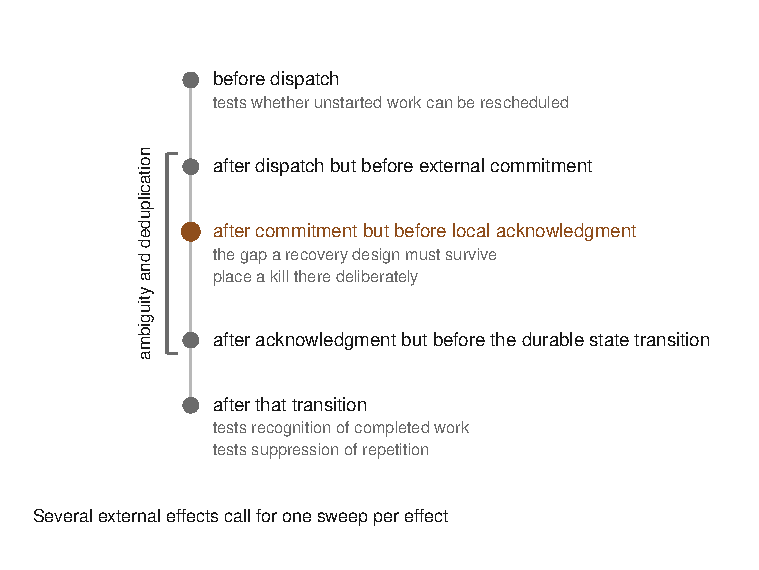
\includegraphics[keepaspectratio,alt={Five lifecycle kill points test recovery from unstarted work through ambiguous commitment gaps to durable completion, including recognition and suppression of repeated external effects.}]{figures/ch09-kill-points.pdf}}
\caption{Five lifecycle kill points test recovery from unstarted work through ambiguous commitment gaps to durable completion, including recognition and suppression of repeated external effects.}
\end{figure}

Each external effect requires a deliberate kill between external commitment and local acknowledgment.

Calls that can hang or return partially add another fault class. Interrupt the connection, inject a retryable response, delay the response beyond the worker heartbeat, and deliver a late response after the retry has begun. The runtime must distinguish a request known not to have executed from one whose status is uncertain. Treating both as ordinary retryable failures converts transport ambiguity into duplicated effects.

Redeployment adds versioned state to the protocol. Kill or replace a worker while a run remains active, then resume it with patched code. The event schema, serialized state, and deterministic replay path may each cross a compatibility boundary. A restart that succeeds with the same binary does not test this case. The configuration record should therefore identify both the pre-fault version and the recovery version.

History growth is another boundary condition. A short demonstration may avoid replay costs, rollover behavior, and compaction defects that appear only after many events. Run beyond the runtime's history rollover or compaction threshold and inject faults on both sides of that boundary.

Compaction replaces detailed working history with a condensed representation so the run remains within its history or context budget. The companion pattern on bounding replay history addresses the architectural response. The experiment determines whether the current boundary behaves as intended.

The fault menu should ultimately come from observed production failures rather than from what the harness can inject conveniently. Worker kills are reproducible and severe, but they do not cover slow storage, stale leases, delayed acknowledgments, partial network partitions, quota errors, or malformed persisted state.

The companion catalog's realistic-fault-menu pattern develops the fuller construction method. The narrower requirement here is to publish the menu so readers can see which failures the recovery claim includes and which it excludes.

\section{Keep the result attached to its envelope}\label{keep-the-result-attached-to-its-envelope}

My kill demonstration, a \textbf{local artifact}, illustrates the protocol without extending the literature evidence. In one run, the worker was killed during an activity after a retryable fault had already been injected. The recovered execution passed all 13 invariant checks. The interrupted activity resumed after a heartbeat-timeout retry, reused a cached result, and produced output identical to the clean reference by content hash.

Thirteen of thirteen is a satisfying result, but it describes one kill placement under one configuration.

I can conclude that the running system exhibited the specified invariants in that trial. I cannot conclude that the engine is generally fault tolerant, that another activity would recover through the same path, or that a different software version would preserve the result. Vogel et al.~(2024) justify that restraint: recovery comparisons changed when configuration and recurring faults were measured directly.

\Needspace{5\baselineskip}

My publish-gate protocol, also a \textbf{local artifact}, defines a broader intended experiment. Its first gate injects a failure in continuous integration at a randomized kill point. The fault matrix includes:

\begin{itemize}
\tightlist
\item
  a kill during a model call;
\item
  a kill inside the execute-then-log gap;
\item
  redeployment with patched code while a run remains active; and
\item
  execution beyond three times the history-rollover threshold.
\end{itemize}

Randomization broadens the sampled placement. It does not replace a fixed sweep across named high-risk intervals.

These artifacts support no comparison among workflow engines. I never ran the comparison sweep, and the non-naive adapters remain specification stubs. There are therefore no author-generated comparative measurements to report. An interface diagram containing several adapters can resemble an experiment even when no workload has passed through them.

\Needspace{5\baselineskip}

Every published result should carry the configuration that produced it. Record:

\begin{itemize}
\tightlist
\item
  runtime and engine versions;
\item
  deployment topology;
\item
  persistence settings;
\item
  checkpoint interval;
\item
  retry policy;
\item
  heartbeat and timeout values;
\item
  resource limits;
\item
  workload shape and concurrency;
\item
  input rate;
\item
  external-service behavior;
\item
  fault-injector version;
\item
  kill-point definition; and
\item
  metric definitions.
\end{itemize}

Preserve the typed trace, or an appropriately redacted derivative, so another investigator can reconstruct the event order. Without this envelope, a recovery number is difficult to interpret and cannot be reproduced closely.

Results also age as the stack changes. A new scheduler, storage client, default timeout, or checkpoint implementation can alter fault detection and state restoration without changing the architecture diagram. A passing experiment establishes behavior only inside the tested envelope. Repeat it after changes that affect persistence, concurrency, retries, version compatibility, external calls, or resource allocation.

Correctness, reliability, and performance should remain separate in the report. The absence of duplicate effects and missing state is a correctness result for a particular trial. The frequency with which those properties hold across injections is a reliability measurement. Recovery time, latency, and throughput are performance measurements.

Resource use and additional model calls belong to cost. An operator's ability to understand the failure and initiate recovery safely belongs to usability. One combined recovery score conceals which property failed.

A recovery system may also need to withhold action when it cannot classify a failure safely. The companion pattern on diagnosing before gating recovery addresses that policy. Another companion pattern asks whether recovery remains invisible to downstream observers except as monotonic progress. Neither property follows from a successful restart, so I exclude both from the basic pass criterion unless the system claims them explicitly.

\section{A protocol for trusting recovery}\label{a-protocol-for-trusting-recovery}

Before accepting a recovery claim about an agent runtime, I look for two linked artifacts.

The first is a durably persisted typed event stream that distinguishes model calls, tool dispatch and completion, environment changes, external commitments, and state transitions. I begin with the shared OpenTelemetry GenAI conventions, then add explicit state, branch, persistence, and effect fields where the workload requires them. Every agent action identifies its owner, and every tool call can be joined to the reasoning step and session that authorized it.

The second artifact is a fault-injection result produced under representative load. I run a clean control, kill a worker from inside an active step, and place at least one kill between an external effect and its durable completion record. I repeat injections within continuing runs and across independent runs because the first restart does not characterize later recovery.

The harness must confirm that the intended kill occurred, observe recovery without supplying recovery state, and exercise a naive negative control expected to duplicate effects.

\Needspace{5\baselineskip}

I measure recovery time between declared application events rather than between process death and process restart. I retain:

\begin{itemize}
\tightlist
\item
  post-recovery throughput and latency;
\item
  invariant outcomes;
\item
  duplicate and missing effects;
\item
  recovery behavior by failure ordinal; and
\item
  output or state equivalence against the clean control.
\end{itemize}

When exact equivalence is impossible, I state which properties were constrained and which outputs remain nondeterministic. A pass means only that the runtime met those conditions in the tested trials.

The fault menu and complete configuration remain attached to the result. Together they define the envelope within which the claim is valid and provide the basis for repeating the experiment after a version or deployment change. A reader should be able to determine which intervals were struck, which faults were omitted, how behavior changed across recurring failures, and which measurements separated correctness from reliability, performance, and cost.

This protocol does not establish that an engine is universally reliable. It supports a narrower and more useful statement:

\begin{quote}
Under a recorded workload and configuration, with specified faults injected at specified boundaries, the runtime recovered with measured behavior and preserved the named invariants.
\end{quote}

That claim can be challenged, repeated, and revised when the system changes.

A trace detailed enough to replay is also the artifact a person reads when recovery fails. Even a complete trace, however, does not establish which action caused the failure or how a person can defend that attribution.

\section*{Sources and evidence}

\textbf{Make every run a structured, replayable trace}

\begin{itemize}
\tightlist
\item
  Directional evidence: Shepherd runtime substrate (Yu et al.~2026, arXiv:2605.10913); companion material named in the same synthesis without a paper identifier: OpenTelemetry GenAI conventions (CNCF 2025).
\item
  Directional evidence: AgentSight eBPF observability (Zheng et al.~2025, arXiv:2508.02736).
\item
  Directional evidence: Chan, A., et al.~(2024), ``Visibility into AI Agents,'' ACM FAccT 2024, arXiv:2401.13138.
\end{itemize}

\textbf{Benchmark recovery with fault injection}

\begin{itemize}
\tightlist
\item
  Strong evidence: Vogel et al.~(2024), ``A Comprehensive Benchmarking Analysis of Fault Recovery in Stream Processing Frameworks,'' arXiv:2404.06203 (JSS line).
\end{itemize}

Author-system cases are narrative illustration, not evidence. The kill demonstration and publish-gate protocol are local artifacts.
